\documentclass[10pt,a4paper]{article}
\usepackage[top=15mm,bottom=17mm,left=18mm,right=18mm,headheight=13pt,headsep=5mm]{geometry}
\usepackage[T1]{fontenc}
\usepackage{lmodern}
\usepackage{amsmath,amssymb,graphicx,booktabs,longtable,array,calc,xcolor}
\usepackage{fancyhdr,titlesec,caption,listings,microtype,float}
\usepackage[hidelinks]{hyperref}
\hypersetup{colorlinks=true,allcolors=black,pdftitle={EN3160 Assignment 3: Neural Networks},pdfauthor={Dilhan W.A.}}
\pagestyle{fancy}\fancyhf{}
\fancyhead[L]{\small EN3160 -- Assignment 03}
\fancyhead[R]{\small 230145E}
\fancyfoot[C]{\small\thepage}
\renewcommand{\headrulewidth}{0.4pt}
\setlength{\parindent}{0pt}\setlength{\parskip}{4pt}
\setlength{\emergencystretch}{3em}
\setlength{\tabcolsep}{4pt}
\renewcommand{\arraystretch}{1.13}
\providecommand{\tightlist}{\setlength{\itemsep}{0pt}\setlength{\parskip}{0pt}}
\newcommand{\passthrough}[1]{#1}
\titleformat{\section}{\large\bfseries}{}{0em}{}
\titleformat{\subsection}{\normalsize\bfseries}{}{0em}{}
\titleformat{\subsubsection}{\normalsize\bfseries}{}{0em}{}
\titlespacing*{\section}{0pt}{9pt}{5pt}
\titlespacing*{\subsection}{0pt}{7pt}{4pt}
\captionsetup{font=footnotesize,labelfont=bf}
\lstset{basicstyle=\ttfamily\scriptsize,keywordstyle=\bfseries,commentstyle=\itshape,
 stringstyle=\ttfamily,frame=tb,rulecolor=\color{black},showstringspaces=false,
 breaklines=true,columns=fullflexible,keepspaces=true,aboveskip=5pt,belowskip=5pt,
 framesep=3pt,language=Python}
\color{black}
\begin{document}
\thispagestyle{plain}
\begin{minipage}[c]{.13\linewidth}

\includegraphics[height=22mm]{../assets/uom_logo.png}
\end{minipage}\hfill
\begin{minipage}[c]{.84\linewidth}
{\small\bfseries University of Moratuwa, Sri Lanka}\par
{\footnotesize Department of Electronic \& Telecommunication Engineering}\par
\vspace{3pt}
{\Large\bfseries EN3160 -- Neural Networks}\par
{\small Assignment 03\quad$\vert$\quad Dilhan W.A.\quad$\vert$\quad 230145E}\par
{\footnotesize October 19, 2026}
\end{minipage}
\par\vspace{5pt}\hrule\vspace{4pt}
{\footnotesize\textbf{Repository:} \url{https://github.com/ahesh-dilhan/en3160-assignment-03}}\par

This notebook presents three full-data experiments, with the implementation, recorded learning curves, confusion matrices, and interpretation of the final models.

\subsection{Experimental protocol}\label{experimental-protocol}

All runs use seed \textbf{230145} and the complete standard splits: CIFAR-10 50,000/10,000; MNIST 60,000/10,000; Hymenoptera 244/153 train/validation. Neither CIFAR-10 nor MNIST is subsampled. The reported training metrics are measured after each epoch, with dropout disabled and batch normalization in evaluation mode. They are not the running averages of training minibatches.

The final scheduled checkpoint is reported for every model: epoch 10 for Questions 1--2 and epoch 25 for Question 3. Curves on held-out data are plotted as requested, but they are not used to tune the settings or choose checkpoints. This is a single fixed-seed comparison, not a claim of statistical significance.

\par\noindent\begin{minipage}{\linewidth}
\begin{lstlisting}[language={}]
Recorded runtime: {'torch': '2.6.0+cu124', 'torchvision': '0.21.0+cu124', 'numpy': '2.5.4', 'device': 'NVIDIA GeForce RTX 2050', 'cuda': '12.4', 'seed': 230145, 'threads': 6}
\end{lstlisting}
\end{minipage}\par

\par\noindent\begin{minipage}{\linewidth}
\begin{lstlisting}[language={}]
CIFAR10 | exact pixel hashes shared across official splits: 0
MNIST | exact pixel hashes shared across official splits: 0
Hymenoptera | exact pixel hashes shared across official splits: 0
\end{lstlisting}
\end{minipage}\par

Input checks verify image shapes, uint8 ranges, class counts, readable insect images, and exact pixel hashes across the official splits. Exact matches are reported transparently; the specified standard splits are retained unchanged. CIFAR-10 uses the byte-identical MIT Open Learning archive mirror, pinned to a revision and checked against the canonical archive MD5, because the original host was unreachable during preparation.

\par\noindent\begin{minipage}{\linewidth}\centering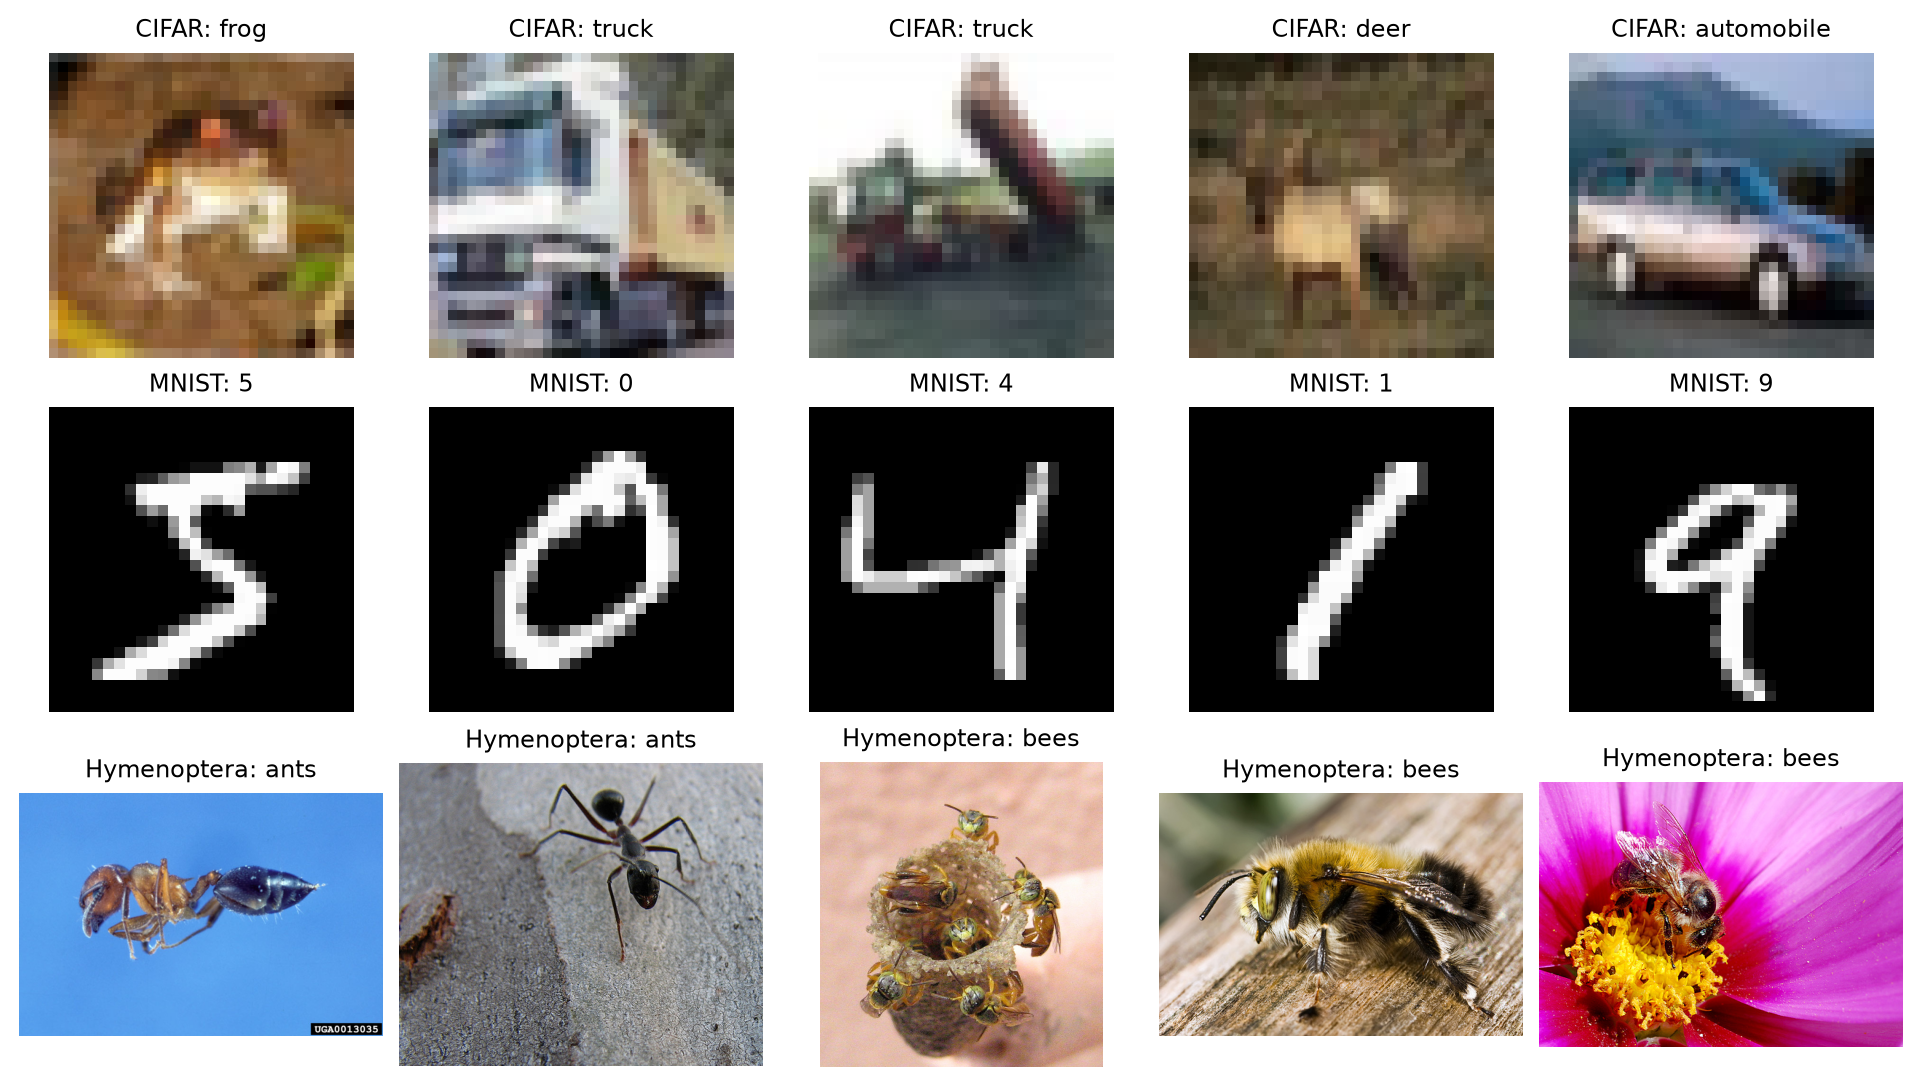
\includegraphics[width=\linewidth,height=.56\textheight,keepaspectratio]{notebook_images/figure_01.png}\par

\emph{Figure 1. Actual training images from the three datasets. Natural image colours are preserved; MNIST is originally grayscale.}

\end{minipage}\par

\clearpage
\subsection{1. CIFAR-10 with manually computed backpropagation}\label{cifar-10-with-manually-computed-backpropagation}

\subsubsection{Architecture and loss}\label{architecture-and-loss}

A normalized RGB image is flattened to \(x\in\mathbb{R}^{3072}\). The new hidden layer contains exactly 100 sigmoid units, followed by ten output logits:

\[H=\sigma(XW_1+b_1),\qquad Z=HW_2+b_2.\]

For batch size \(N\), the numerically stable mean cross-entropy is

\[L=-\frac{1}{N}\sum_{i=1}^{N}\left[Z_{i,y_i}-\operatorname{logsumexp}_k Z_{ik}\right].\]

Let \(P=\operatorname{softmax}(Z)\) and \(Y\) be one-hot targets. The analytic gradients are

\[G=(P-Y)/N,\quad \nabla W_2=H^T G,\quad \nabla b_2=\sum_i G_i,\] \[D=(GW_2^T)\odot H\odot(1-H),\quad \nabla W_1=X^T D,\quad \nabla b_1=\sum_i D_i.\]

All four gradients are calculated before either weight matrix is updated. Training uses tensor operations and manual SGD, without \passthrough{\lstinline!backward()!}, \passthrough{\lstinline!torch.optim!}, or autograd. Autograd is used only as an independent gradient oracle in a small unit test.

\par\noindent\begin{minipage}{\linewidth}
\begin{lstlisting}
def loss_and_gradients(self, x, y):
    logits, h = self.forward(x)
    log_prob = logits - torch.logsumexp(logits, dim=1, keepdim=True)
    loss = -log_prob[torch.arange(len(y), device=y.device), y].mean()
    dz = log_prob.exp()
    dz[torch.arange(len(y), device=y.device), y] -= 1
    dz /= len(y)
    dw2, db2 = h.T @ dz, dz.sum(0)
    dh = (dz @ self.w2.T) * h * (1 - h)
    dw1, db1 = x.T @ dh, dh.sum(0)
    return loss, [dw1, db1, dw2, db2]
\end{lstlisting}
\end{minipage}\par

\subsubsection{Training settings and implementation choices}\label{training-settings-and-implementation-choices}

The supplied listing's CIFAR-10 normalization, batch size \textbf{50}, zero regularization, and epoch decay \textbf{0.9} are retained. There are \textbf{10 epochs}. The initial learning rate is \textbf{0.1} and the weights use fan-in normal initialization. These two settings replace the listing's \passthrough{\lstinline!2e-6!} learning rate and \passthrough{\lstinline!1e-5!} weight standard deviation, which are poorly scaled for a new sigmoid/mean-cross-entropy model. This is a disclosed implementation choice; no claim is made that those original settings would produce the same results.

For every batch, \passthrough{\lstinline!ManualMLP.step!} applies \passthrough{\lstinline!parameter -= learning\_rate * gradient!}. The sigmoid derivative is evaluated from its cached activation, and log-sum-exp prevents overflow when computing the loss.

\par\noindent\begin{minipage}{\linewidth}
\begin{lstlisting}
if RUN_TRAINING:
    cifar(torch.device('cuda' if torch.cuda.is_available() else 'cpu'))
    refresh_figures('q1')
else:
    print('Using the completed full-data, 10-epoch manual-gradient run.')
result_table(['cifar_manual'], ['Manual sigmoid MLP'])
\end{lstlisting}
\end{minipage}\par

\par\noindent\begin{minipage}{\linewidth}
\begin{lstlisting}[language={}]
Using the completed full-data, 10-epoch manual-gradient run.
\end{lstlisting}
\end{minipage}\par

{\def\LTcaptype{table} % do not increment counter
\begin{longtable}[]{@{}
  >{\raggedright\arraybackslash}p{(\linewidth - 10\tabcolsep) * \real{0.1304}}
  >{\raggedleft\arraybackslash}p{(\linewidth - 10\tabcolsep) * \real{0.1739}}
  >{\raggedleft\arraybackslash}p{(\linewidth - 10\tabcolsep) * \real{0.1739}}
  >{\raggedleft\arraybackslash}p{(\linewidth - 10\tabcolsep) * \real{0.1739}}
  >{\raggedleft\arraybackslash}p{(\linewidth - 10\tabcolsep) * \real{0.1739}}
  >{\raggedleft\arraybackslash}p{(\linewidth - 10\tabcolsep) * \real{0.1739}}@{}}
\toprule\noalign{}
\begin{minipage}[b]{\linewidth}\raggedright
Model
\end{minipage} & \begin{minipage}[b]{\linewidth}\raggedleft
Epochs
\end{minipage} & \begin{minipage}[b]{\linewidth}\raggedleft
Train loss
\end{minipage} & \begin{minipage}[b]{\linewidth}\raggedleft
Train accuracy
\end{minipage} & \begin{minipage}[b]{\linewidth}\raggedleft
Test loss
\end{minipage} & \begin{minipage}[b]{\linewidth}\raggedleft
Test accuracy
\end{minipage} \\
\midrule\noalign{}
\endhead
\bottomrule\noalign{}
\endlastfoot
Manual sigmoid MLP & 10 & 1.3728 & 53.13\% & 1.5060 & 47.77\% \\
\end{longtable}
}

\par\noindent\begin{minipage}{\linewidth}\centering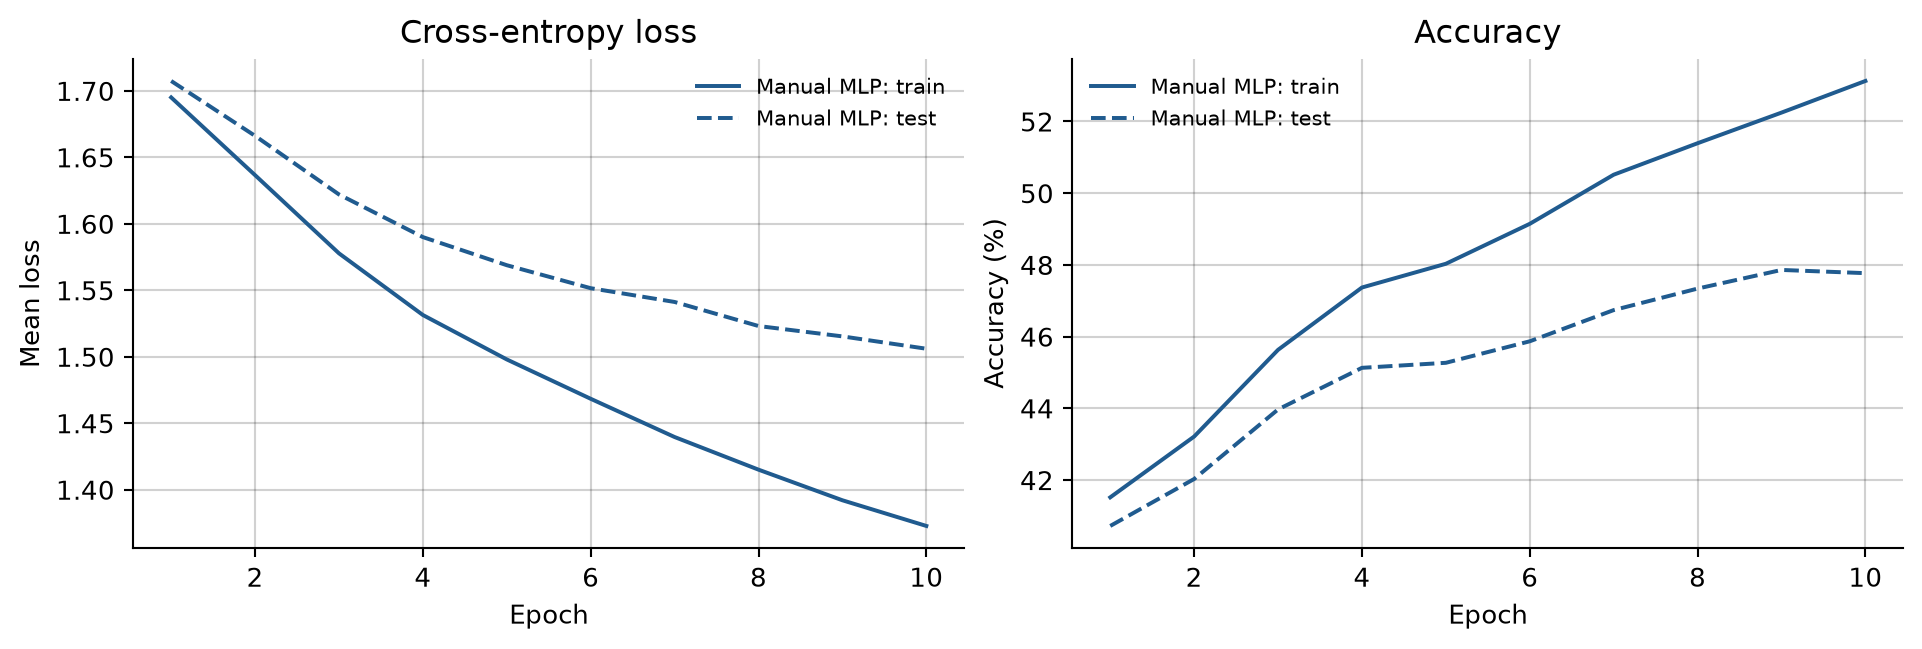
\includegraphics[width=\linewidth,height=.56\textheight,keepaspectratio]{notebook_images/figure_02.png}\par

\emph{Figure 2. Full training and test splits evaluated after each of the ten epochs; mean cross-entropy and accuracy.}

\end{minipage}\par

\textbf{Interpretation.} The final network classifies 4,777 of 10,000 test images correctly. The train--test accuracy gap is 5.36 percentage points. A flattened dense model has no convolutional locality or translation-sharing bias. Its ten-epoch result demonstrates the requested manual optimization, while leaving substantial classification error on visually varied natural images. A lower training loss by itself does not establish better generalization.

\subsection{2. MNIST: LeNet-5 and a modern three-layer CNN}\label{mnist-lenet-5-and-a-modern-three-layer-cnn}

\subsubsection{Networks}\label{networks}

\textbf{LeNet-5:} normalized MNIST is padded from 28 x 28 to 32 x 32. The path is Conv(1 -\textgreater{} 6, 5 x 5) -\textgreater{} tanh -\textgreater{} average pool(2) -\textgreater{} Conv(6 -\textgreater{} 16, 5 x 5) -\textgreater{} tanh -\textgreater{} average pool(2) -\textgreater{} 400 -\textgreater{} 120 -\textgreater{} 84 -\textgreater{} 10. The 400 -\textgreater{} 120 dense layer is equivalent to a 5 x 5 convolution on the 16 x 5 x 5 feature maps. The historical RBF output is replaced with ten linear logits and cross-entropy, a standard classification adaptation.

\par\noindent\begin{minipage}{\linewidth}
\begin{lstlisting}
class LeNet5(nn.Module):
    """32x32 padded MNIST, tanh and average pooling, linear CE head."""
    def __init__(self):
        super().__init__()
        self.features = nn.Sequential(
            nn.Conv2d(1, 6, 5), nn.Tanh(), nn.AvgPool2d(2),
            nn.Conv2d(6, 16, 5), nn.Tanh(), nn.AvgPool2d(2),
        )
        self.classifier = nn.Sequential(
            nn.Flatten(), nn.Linear(16 * 5 * 5, 120), nn.Tanh(),
            nn.Linear(120, 84), nn.Tanh(), nn.Linear(84, 10),
        )

    def forward(self, x):
        return self.classifier(self.features(x))
\end{lstlisting}
\end{minipage}\par

\textbf{Modern CNN:} exactly three 3 x 3 convolutions (32, 64, 128 channels), each followed by batch normalization, ReLU, 2 x 2 max pooling, and spatial dropout (0.10, 0.15, 0.20). A further dropout of 0.30 precedes the final linear classifier.

\par\noindent\begin{minipage}{\linewidth}
\begin{lstlisting}
class ModernCNN(nn.Module):
    """Exactly three convolution layers, each followed by batch norm."""
    def __init__(self):
        super().__init__()
        layers = []
        for incoming, outgoing, drop in [(1, 32, .10), (32, 64, .15), (64, 128, .20)]:
            layers += [nn.Conv2d(incoming, outgoing, 3, padding=1, bias=False),
                       nn.BatchNorm2d(outgoing), nn.ReLU(), nn.MaxPool2d(2),
                       nn.Dropout2d(drop)]
        self.features = nn.Sequential(*layers)
        self.classifier = nn.Sequential(nn.Flatten(), nn.Dropout(.3),
                                        nn.Linear(128 * 4 * 4, 10))

    def forward(self, x):
        return self.classifier(self.features(x))
\end{lstlisting}
\end{minipage}\par

\subsubsection{Matched training conditions}\label{matched-training-conditions}

Both networks use all 60,000 training images, \textbf{10 epochs}, batch size \textbf{128}, Adam with learning rate \textbf{0.001}, betas (0.9, 0.999), no weight decay, no learning rate schedule, and no data augmentation. Normalization is \passthrough{\lstinline!(x/255-0.1307)/0.3081!}. Padding is the normalized value of a black pixel, not an unnormalized zero. The seed and an independent shuffle generator provide the exact same minibatch order to both architectures. The architecture, parameter count, and inherent dropout/BN behavior are the intended differences.

\par\noindent\begin{minipage}{\linewidth}
\begin{lstlisting}
# Core loop used for each MNIST architecture (data tensors are on the device).
from src.experiments import evaluate_tensor
def train_mnist_model(model, x, y, x_test, y_test):
    optimizer = torch.optim.Adam(model.parameters(), lr=0.001)
    generator = torch.Generator(device=x.device).manual_seed(230145)
    for epoch in range(10):
        model.train()
        order = torch.randperm(len(y), generator=generator, device=x.device)
        for indices in order.split(128):
            optimizer.zero_grad(set_to_none=True)
            loss = nn.functional.cross_entropy(model(x[indices]), y[indices])
            loss.backward()
            optimizer.step()
        train_metrics, _ = evaluate_tensor(model, x, y, batch_size=256)
        test_metrics, _ = evaluate_tensor(model, x_test, y_test, batch_size=256)
        print(epoch + 1, train_metrics, test_metrics)
\end{lstlisting}
\end{minipage}\par

\par\noindent\begin{minipage}{\linewidth}
\begin{lstlisting}
if RUN_TRAINING:
    mnist(torch.device('cuda' if torch.cuda.is_available() else 'cpu'))
    refresh_figures('q2')
else:
    print('Using both completed full-data, 10-epoch MNIST runs.')
result_table(['lenet5','modern_cnn'], ['LeNet-5','Modern CNN'])
for name in ['lenet5','modern_cnn']:
    s=summary(name)
    print(name, 'parameters:', s['config']['parameters'],
          '| test correct:', s['test']['correct'], '/', s['test']['count'])
\end{lstlisting}
\end{minipage}\par

\par\noindent\begin{minipage}{\linewidth}
\begin{lstlisting}[language={}]
Using both completed full-data, 10-epoch MNIST runs.
\end{lstlisting}
\end{minipage}\par

{\def\LTcaptype{table} % do not increment counter
\begin{longtable}[]{@{}
  >{\raggedright\arraybackslash}p{(\linewidth - 10\tabcolsep) * \real{0.1304}}
  >{\raggedleft\arraybackslash}p{(\linewidth - 10\tabcolsep) * \real{0.1739}}
  >{\raggedleft\arraybackslash}p{(\linewidth - 10\tabcolsep) * \real{0.1739}}
  >{\raggedleft\arraybackslash}p{(\linewidth - 10\tabcolsep) * \real{0.1739}}
  >{\raggedleft\arraybackslash}p{(\linewidth - 10\tabcolsep) * \real{0.1739}}
  >{\raggedleft\arraybackslash}p{(\linewidth - 10\tabcolsep) * \real{0.1739}}@{}}
\toprule\noalign{}
\begin{minipage}[b]{\linewidth}\raggedright
Model
\end{minipage} & \begin{minipage}[b]{\linewidth}\raggedleft
Epochs
\end{minipage} & \begin{minipage}[b]{\linewidth}\raggedleft
Train loss
\end{minipage} & \begin{minipage}[b]{\linewidth}\raggedleft
Train accuracy
\end{minipage} & \begin{minipage}[b]{\linewidth}\raggedleft
Test loss
\end{minipage} & \begin{minipage}[b]{\linewidth}\raggedleft
Test accuracy
\end{minipage} \\
\midrule\noalign{}
\endhead
\bottomrule\noalign{}
\endlastfoot
LeNet-5 & 10 & 0.0128 & 99.60\% & 0.0396 & 98.78\% \\
Modern CNN & 10 & 0.0124 & 99.61\% & 0.0252 & 99.22\% \\
\end{longtable}
}

\par\noindent\begin{minipage}{\linewidth}
\begin{lstlisting}[language={}]
lenet5 parameters: 61706 | test correct: 9878 / 10000
modern_cnn parameters: 113386 | test correct: 9922 / 10000
\end{lstlisting}
\end{minipage}\par

\par\noindent\begin{minipage}{\linewidth}\centering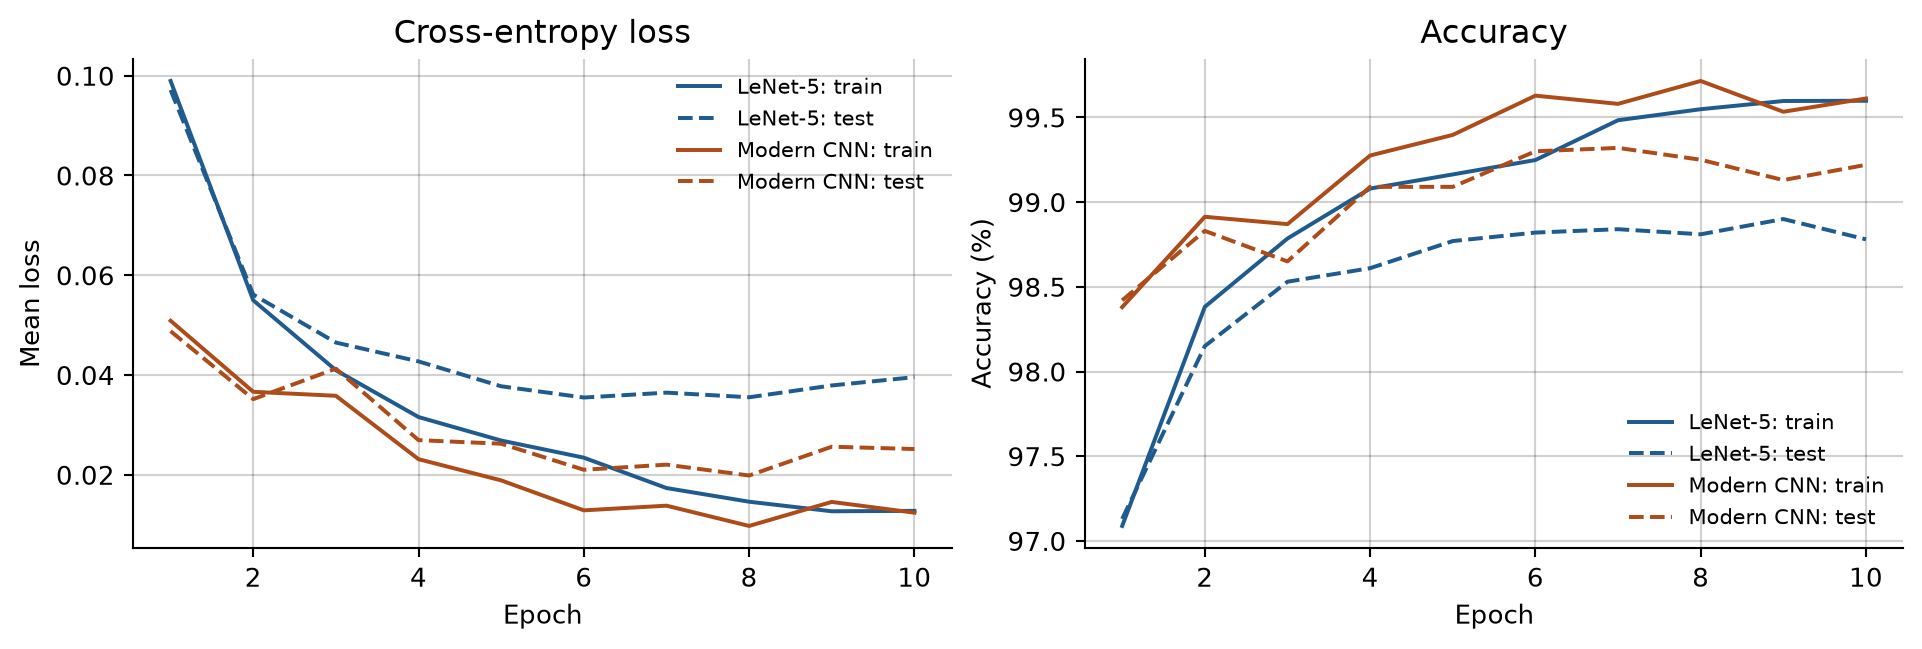
\includegraphics[width=\linewidth,height=.56\textheight,keepaspectratio]{notebook_images/figure_03.png}\par

\emph{Figure 3. Per-epoch train/test loss and accuracy for both networks under the same training conditions. Solid lines: train; dashed lines: test.}

\end{minipage}\par

\par\noindent\begin{minipage}{\linewidth}\centering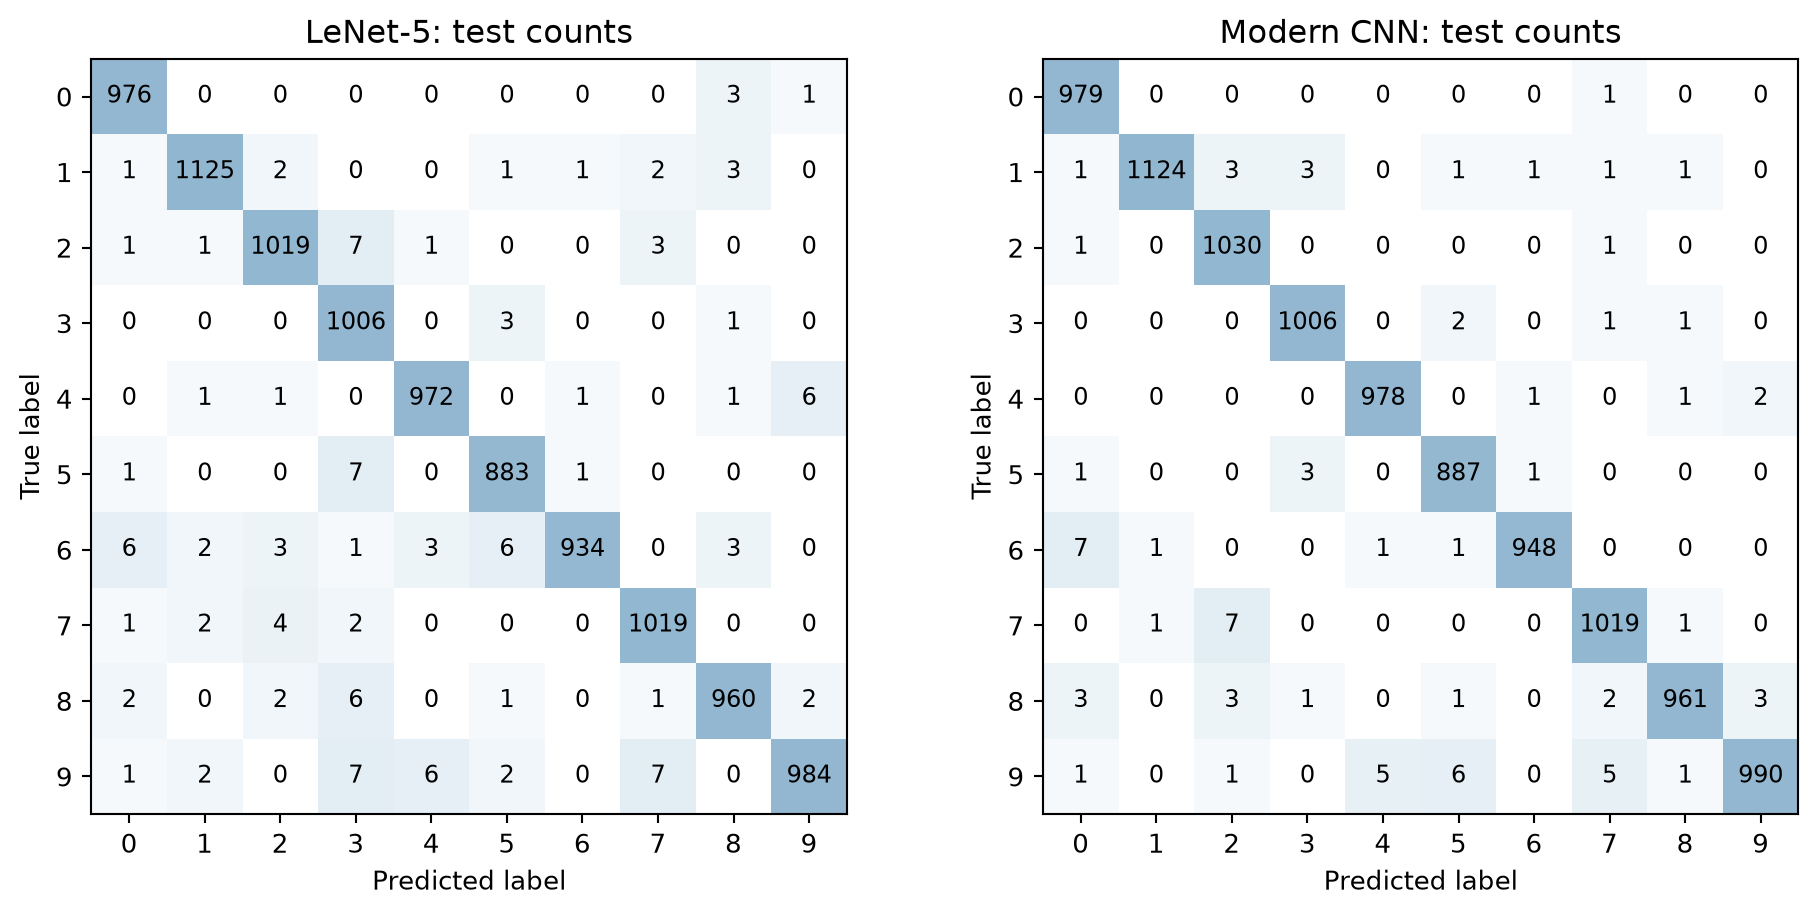
\includegraphics[width=\linewidth,height=.56\textheight,keepaspectratio]{notebook_images/figure_04.png}\par

\emph{Figure 4. Separate test confusion matrices. Rows are true labels and columns are predictions; every displayed number is a count. A log(1+count) colour scale makes small off-diagonal errors visible.}

\end{minipage}\par

\par\noindent\begin{minipage}{\linewidth}\centering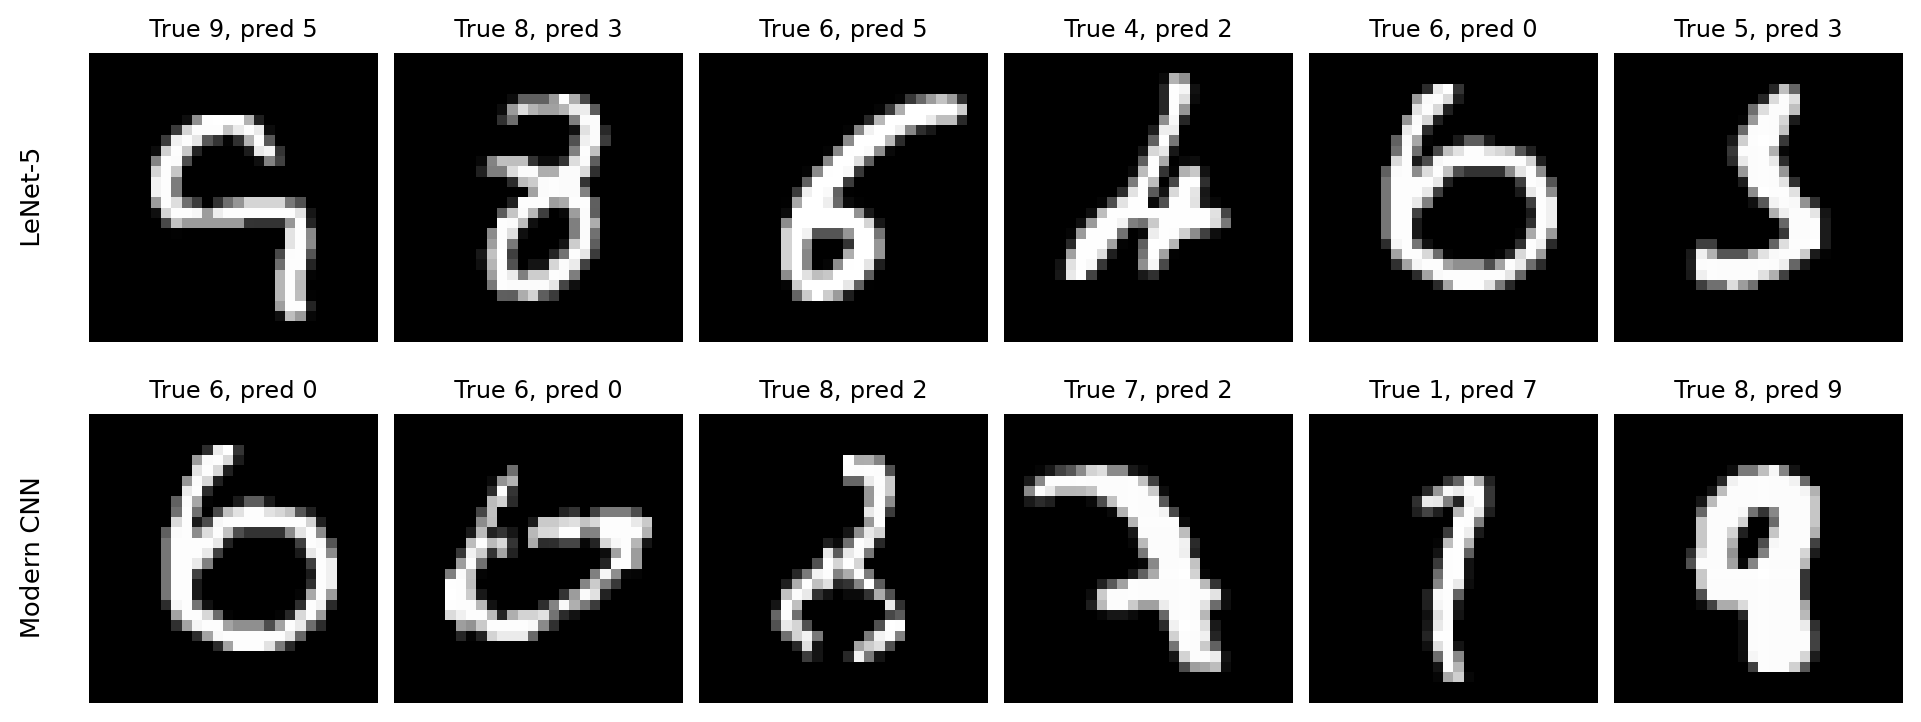
\includegraphics[width=\linewidth,height=.56\textheight,keepaspectratio]{notebook_images/figure_05.png}\par

\emph{Figure 5. The first six test errors in dataset order for each model. These examples are illustrative, not a random estimate of error frequency.}

\end{minipage}\par

\textbf{Comparison.} Modern CNN minus LeNet-5 is \textbf{+0.44 percentage points} in final test accuracy (78 versus 122 errors). The train--test gaps are 0.82 points for LeNet-5 and 0.39 for the modern CNN. The modern network uses 113,386 parameters versus 61,706; training plus evaluation takes 57.8s versus 12.9s in this run. Batch normalization supports stable deeper optimization; dropout regularizes the modern model, while convolutional locality benefits both models. Parameter counts differ, so this compares complete architectures rather than isolating BN or dropout. The loss curves distinguish confidence changes from changes in the number of correct classifications. Some poorly formed digits remain ambiguous, as the error examples show. One seed and ten epochs cannot establish which architecture is universally best.

LeNet-5's test loss falls to about 0.0355 at epoch 6 and rises to 0.0396 at epoch 10 while training loss continues lower, suggesting mild overfitting. The modern CNN also fluctuates late in training rather than improving monotonically. Neither curve is used to replace the prescribed final-epoch checkpoint.

\par\noindent\begin{minipage}{\linewidth}
\begin{lstlisting}[language={}]
lenet5 largest directed confusions: 9 -> 7: 7, 9 -> 3: 7, 2 -> 3: 7
modern_cnn largest directed confusions: 7 -> 2: 7, 6 -> 0: 7, 9 -> 5: 6
\end{lstlisting}
\end{minipage}\par

\subsection{3. Hymenoptera transfer learning with ResNet18}\label{hymenoptera-transfer-learning-with-resnet18}

\subsubsection{Data, preprocessing and two adaptation strategies}\label{data-preprocessing-and-two-adaptation-strategies}

The tutorial dataset has \textbf{244 training images} (123 ants, 121 bees) and \textbf{153 validation images} (70 ants, 83 bees). There is \textbf{no independent test split}. Always predicting bees would give 54.25\% validation accuracy.

Both experiments start from \passthrough{\lstinline!ResNet18\_Weights.IMAGENET1K\_V1!}, trained on ImageNet1K. The original 1000-class head is replaced by a 512 -\textgreater{} 2 linear head. Fine-tuning updates the entire network. Feature extraction freezes every backbone parameter and all batch-normalization running statistics; only the new head is trained.

Training uses RandomResizedCrop(224), horizontal flips, and ImageNet normalization (means 0.485/0.456/0.406, standard deviations 0.229/0.224/0.225). Evaluation uses Resize(256), CenterCrop(224), and the same normalization. Training accuracy here is evaluated with deterministic center crops, not random training augmentations.

Both runs use \textbf{25 epochs}, batch size \textbf{16}, SGD with learning rate \textbf{0.001}, momentum \textbf{0.9}, and StepLR(step\_size=7, gamma=0.1), based on the official tutorial. The final epoch is reported instead of selecting the best validation checkpoint.

\par\noindent\begin{minipage}{\linewidth}
\begin{lstlisting}
from torchvision import models
def initialize_resnet(feature_extractor=False):
    model = models.resnet18(weights=models.ResNet18_Weights.IMAGENET1K_V1)
    if feature_extractor:
        for parameter in model.parameters():
            parameter.requires_grad_(False)
    model.fc = nn.Linear(model.fc.in_features, 2)
    return model

def set_training_mode(model, feature_extractor=False):
    model.train()
    if feature_extractor:
        model.eval()     # Freeze backbone BN running mean and variance too.
        model.fc.train()
\end{lstlisting}
\end{minipage}\par

\par\noindent\begin{minipage}{\linewidth}
\begin{lstlisting}
if RUN_TRAINING:
    transfer(torch.device('cuda' if torch.cuda.is_available() else 'cpu'))
    refresh_figures('q3')
else:
    print('Using both completed full-data, 25-epoch transfer-learning runs.')
result_table(['resnet18_finetune','resnet18_features'],
             ['ResNet18 fine-tuning','ResNet18 fixed features'],split='validation')
for name in ['resnet18_finetune','resnet18_features']:
    s=summary(name)
    print(name, '| trainable parameters:', s['config']['trainable_parameters'],
          '| validation correct:', s['validation']['correct'], '/', s['validation']['count'],
          '| training + evaluation seconds:', round(s['duration_seconds'],1))
\end{lstlisting}
\end{minipage}\par

\par\noindent\begin{minipage}{\linewidth}
\begin{lstlisting}[language={}]
Using both completed full-data, 25-epoch transfer-learning runs.
\end{lstlisting}
\end{minipage}\par

{\def\LTcaptype{table} % do not increment counter
\begin{longtable}[]{@{}
  >{\raggedright\arraybackslash}p{(\linewidth - 10\tabcolsep) * \real{0.1304}}
  >{\raggedleft\arraybackslash}p{(\linewidth - 10\tabcolsep) * \real{0.1739}}
  >{\raggedleft\arraybackslash}p{(\linewidth - 10\tabcolsep) * \real{0.1739}}
  >{\raggedleft\arraybackslash}p{(\linewidth - 10\tabcolsep) * \real{0.1739}}
  >{\raggedleft\arraybackslash}p{(\linewidth - 10\tabcolsep) * \real{0.1739}}
  >{\raggedleft\arraybackslash}p{(\linewidth - 10\tabcolsep) * \real{0.1739}}@{}}
\toprule\noalign{}
\begin{minipage}[b]{\linewidth}\raggedright
Model
\end{minipage} & \begin{minipage}[b]{\linewidth}\raggedleft
Epochs
\end{minipage} & \begin{minipage}[b]{\linewidth}\raggedleft
Train loss
\end{minipage} & \begin{minipage}[b]{\linewidth}\raggedleft
Train accuracy
\end{minipage} & \begin{minipage}[b]{\linewidth}\raggedleft
Validation loss
\end{minipage} & \begin{minipage}[b]{\linewidth}\raggedleft
Validation accuracy
\end{minipage} \\
\midrule\noalign{}
\endhead
\bottomrule\noalign{}
\endlastfoot
ResNet18 fine-tuning & 25 & 0.0323 & 99.59\% & 0.1584 & 94.12\% \\
ResNet18 fixed features & 25 & 0.0763 & 97.54\% & 0.1129 & 96.08\% \\
\end{longtable}
}

\par\noindent\begin{minipage}{\linewidth}
\begin{lstlisting}[language={}]
resnet18_finetune | trainable parameters: 11177538 | validation correct: 144 / 153 | training + evaluation seconds: 94.0
resnet18_features | trainable parameters: 1026 | validation correct: 147 / 153 | training + evaluation seconds: 95.0
\end{lstlisting}
\end{minipage}\par

\par\noindent\begin{minipage}{\linewidth}\centering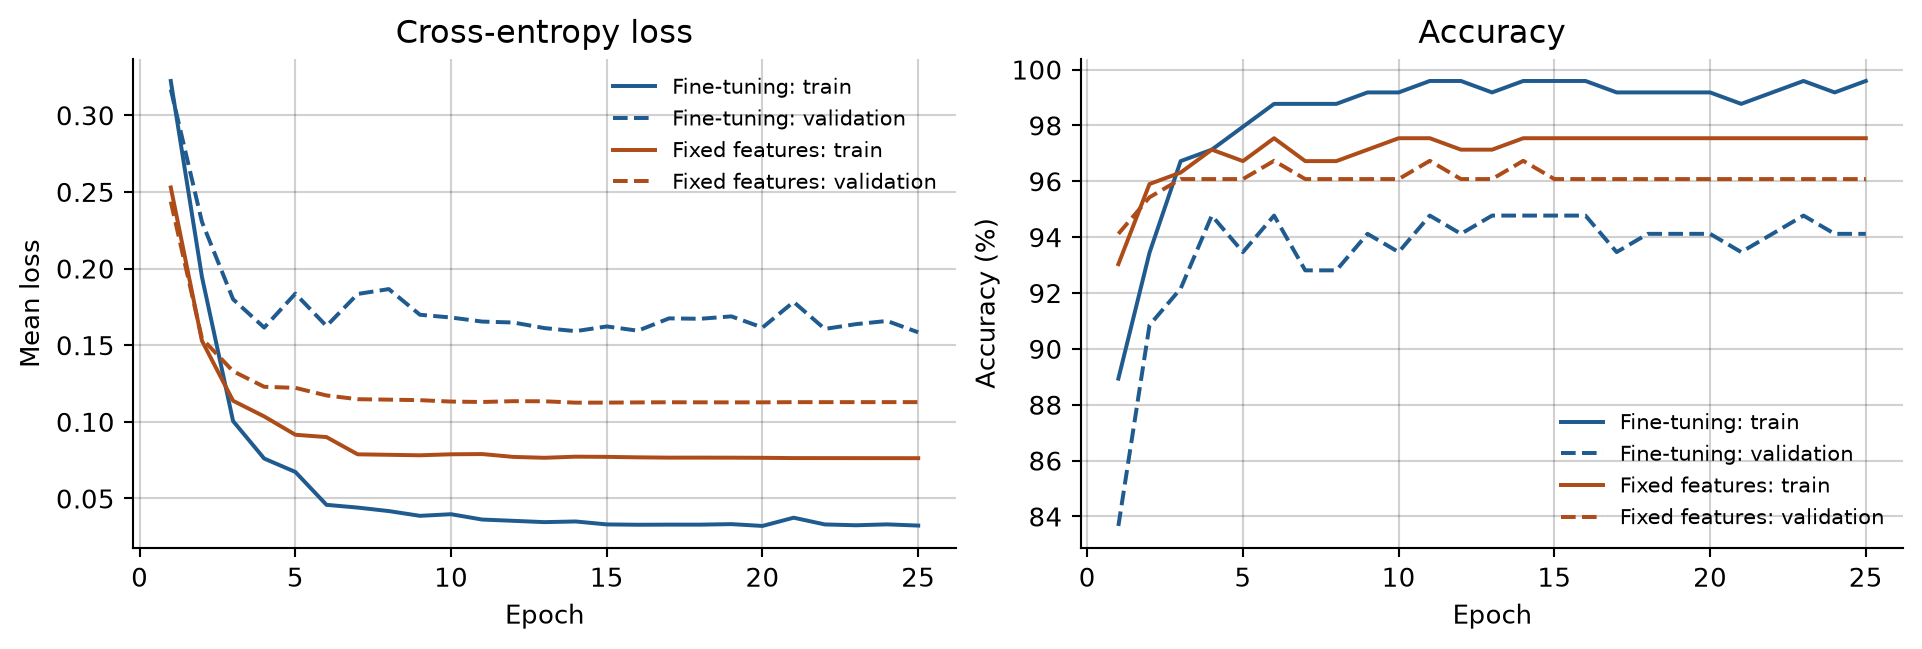
\includegraphics[width=\linewidth,height=.56\textheight,keepaspectratio]{notebook_images/figure_06.png}\par

\emph{Figure 6. Twenty-five-epoch train/validation learning curves. Scheduled reductions occur after epochs 7, 14, and 21.}

\end{minipage}\par

\par\noindent\begin{minipage}{\linewidth}\centering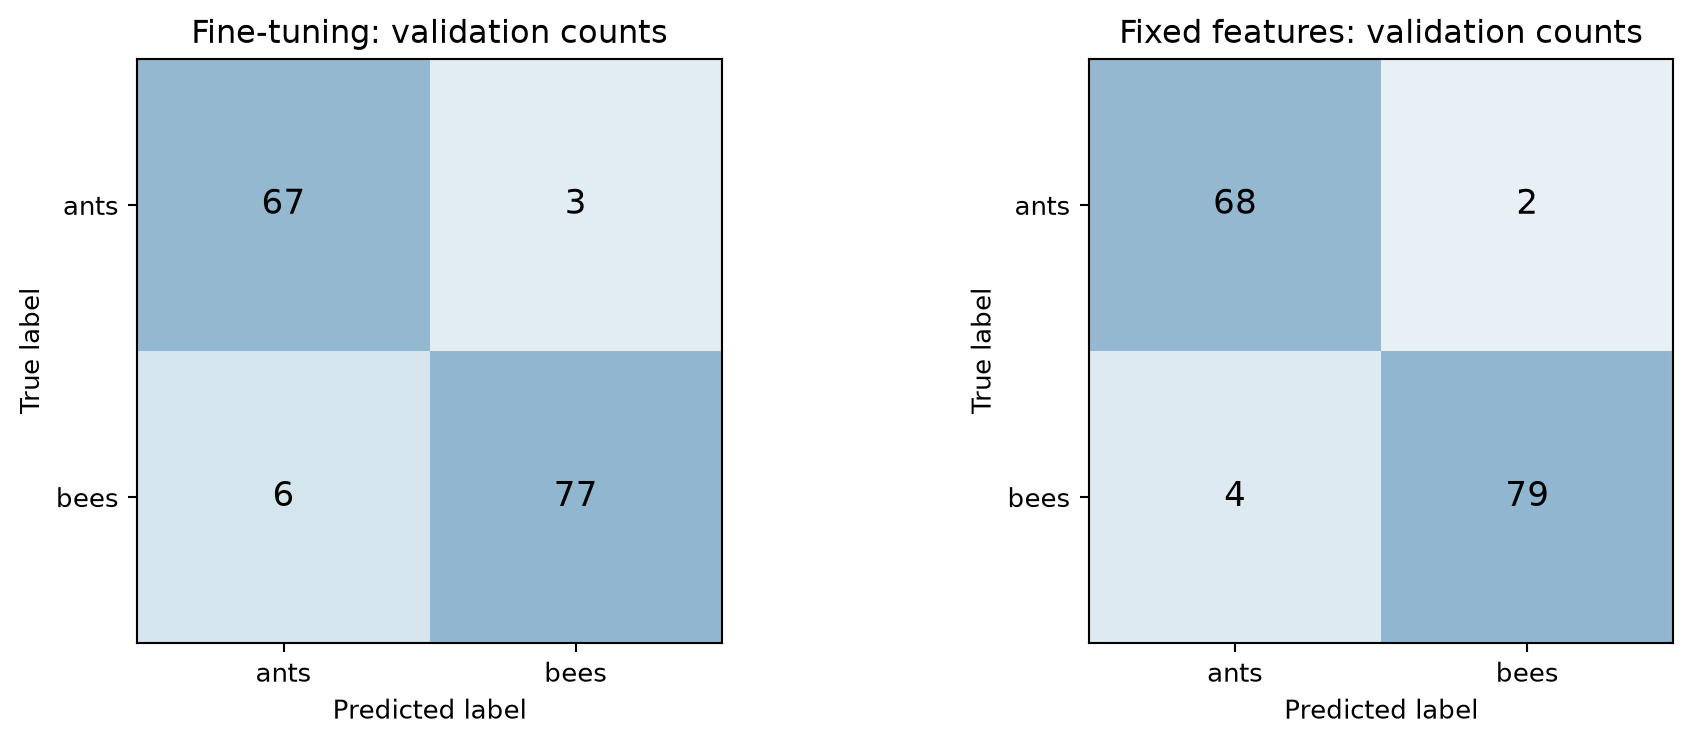
\includegraphics[width=\linewidth,height=.56\textheight,keepaspectratio]{notebook_images/figure_07.png}\par

\emph{Figure 7. Validation confusion matrices for fine-tuning and frozen feature extraction. Every matrix contains all 153 held-out images.}

\end{minipage}\par

\par\noindent\begin{minipage}{\linewidth}\centering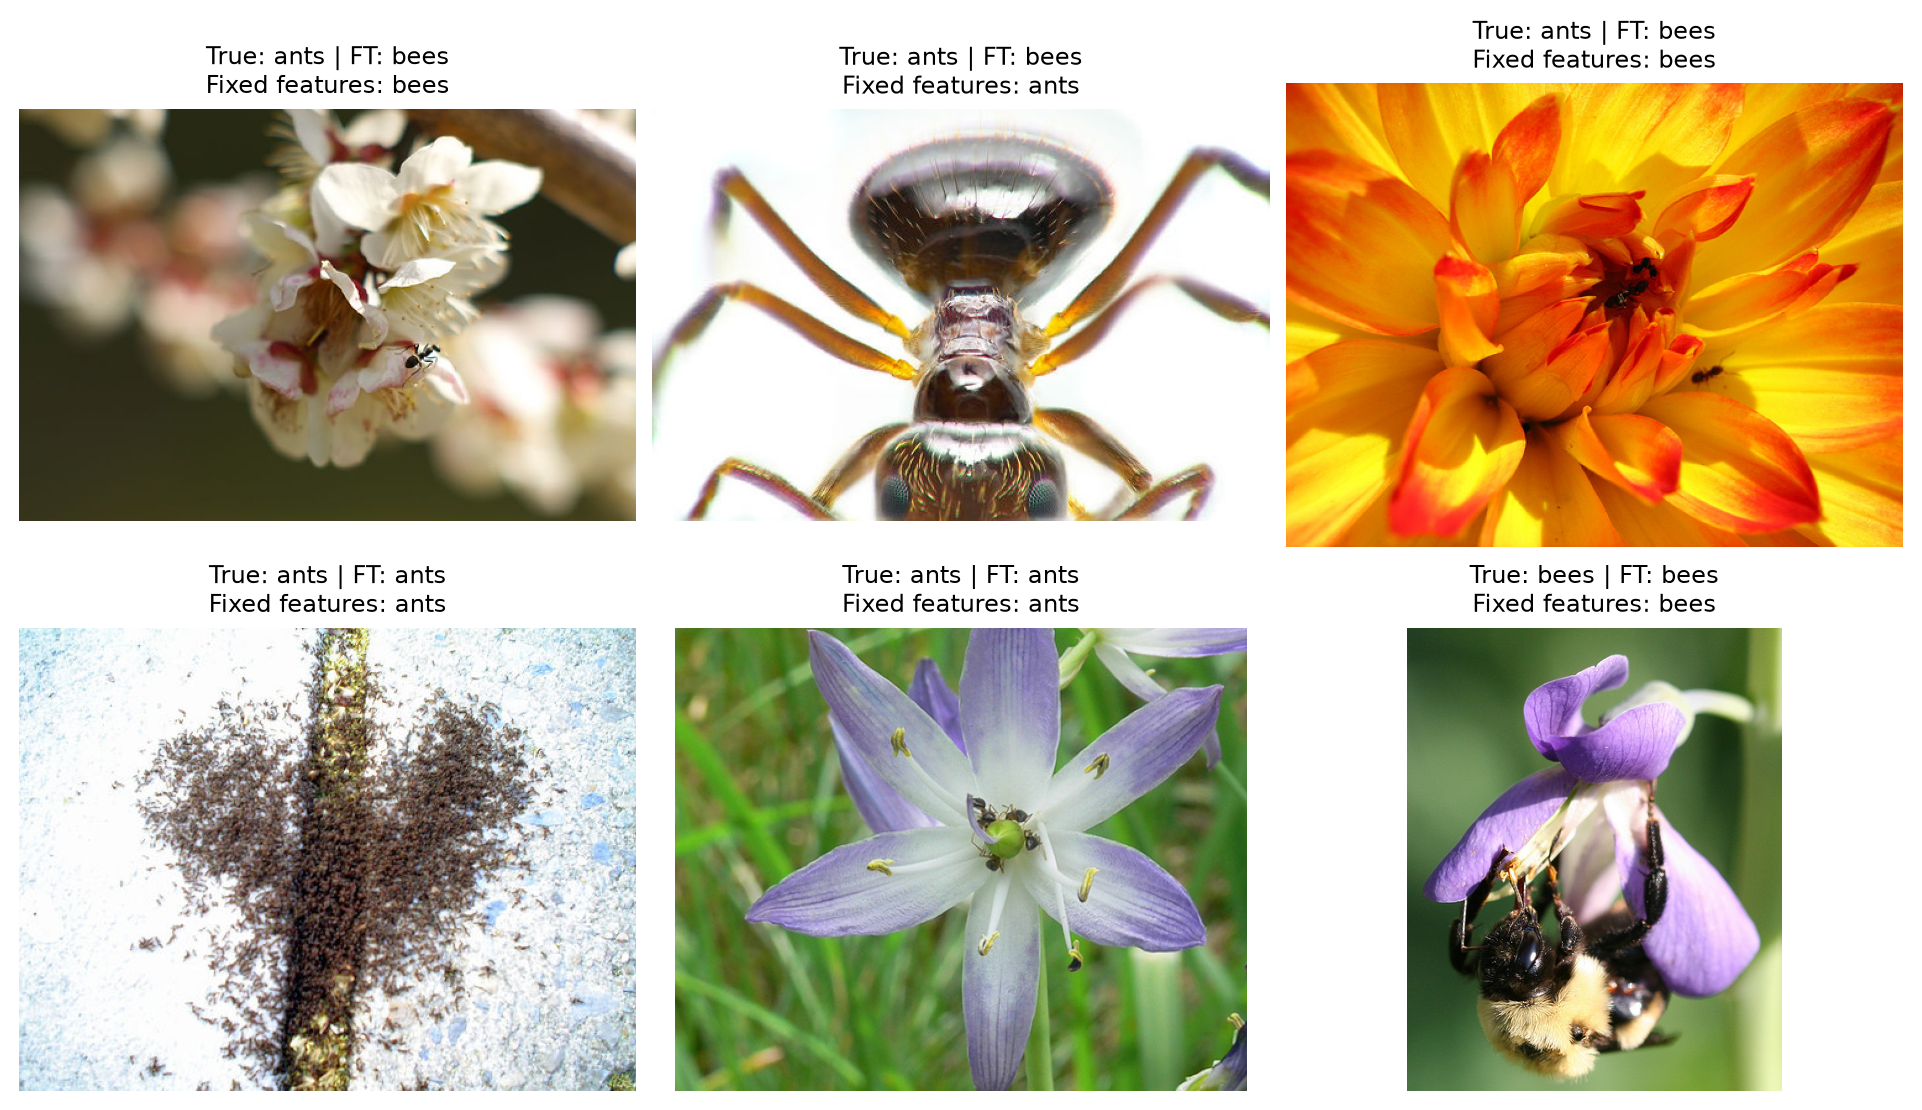
\includegraphics[width=\linewidth,height=.56\textheight,keepaspectratio]{notebook_images/figure_08.png}\par

\emph{Figure 8. Actual validation images: the first three disagreements with ground truth from either model, followed by fixed correct examples. FT denotes fine-tuning; original image colours are retained.}

\end{minipage}\par

\textbf{Interpretation.} Fine-tuning minus fixed features is \textbf{-1.96 percentage points} in final validation accuracy. Fine-tuning gets 144/153 correct; the fixed extractor gets 147/153. One image changes accuracy by about 0.65 percentage points on this small split. Fine-tuning adapts visual features but exposes many more parameters to just 244 training images. A fixed extractor retains ImageNet representations and reduces the optimized parameter count to 1,026, reducing backward computation and the opportunity to overfit. Measured training-plus-evaluation times are 94.0s for fine-tuning and 95.0s for fixed features. These similar totals include input transforms and full-split evaluation, so this run does not demonstrate an end-to-end speed advantage for freezing the backbone. Background context, insect scale, and cropped or partially visible insects can affect either classifier. These are possible explanations, not causal conclusions from six visual examples. No independent test split or repeated-seed uncertainty estimate was supplied, so the comparison is limited to this validation split.

\par\noindent\begin{minipage}{\linewidth}
\begin{lstlisting}[language={}]
resnet18_finetune | ant recall: 95.71% | bee recall: 92.77% | balanced accuracy: 94.24%
resnet18_features | ant recall: 97.14% | bee recall: 95.18% | balanced accuracy: 96.16%
\end{lstlisting}
\end{minipage}\par

\subsection{4. Reproducibility and verification}\label{reproducibility-and-verification}

The executed notebook loads the saved full-training results by default, explicitly printing this choice. Setting \passthrough{\lstinline!RUN\_TRAINING=True!} reruns the actual experiment functions. Training code is in \passthrough{\lstinline!src/models.py!} and \passthrough{\lstinline!src/experiments.py!}; epoch CSVs, prediction arrays, count matrices, input SHA-256 hashes, runtime versions, seeds, checkpoint hashes and figures are retained in the repository. The saved checkpoints allow independent inference without retraining.

The manual-gradient test checks all four analytic gradients against float64 autograd, including repeated class labels. A large-logit case checks loss stability and an SGD step. Other tests verify the required model shapes/layer counts and that the fixed extractor keeps BN statistics unchanged while the classification head receives gradients. The held-out predictions are also regenerated by independently reloading each saved checkpoint and compared with the archived prediction arrays. Confusion-matrix totals, diagonal accuracies, epoch counts, summaries and checkpoint hashes are cross-checked.

Reproduce from the repository root:

\begin{lstlisting}[language=bash]
python -m pip install -r requirements.txt
python -m pytest tests -q
python -m src.experiments --task all
python scripts/verify_results.py
python scripts/verify_checkpoints.py
python scripts/make_figures.py
python scripts/build_notebook.py
python scripts/export_pdf.py
\end{lstlisting}

The notebook PDF is generated through LaTeX, with black document text and rules, a compact university heading on the first content page, and original-colour raster images. No separate cover is used.

\subsubsection{References}\label{references}

\begin{enumerate}
\def\labelenumi{\arabic{enumi}.}
\tightlist
\item
  Ranga Rodrigo. \emph{EN3160 Assignment 3 on Neural Networks}, October 9, 2026. Supplied brief.
\item
  PyTorch. \href{https://docs.pytorch.org/tutorials/beginner/transfer_learning_tutorial.html}{Transfer Learning for Computer Vision Tutorial}.
\item
  \href{https://www.cs.toronto.edu/~kriz/cifar.html}{CIFAR-10 dataset}.
\item
  Torchvision. \href{https://docs.pytorch.org/vision/stable/generated/torchvision.datasets.MNIST.html}{MNIST dataset}.
\item
  Torchvision. \href{https://docs.pytorch.org/vision/stable/models/generated/torchvision.models.resnet18.html}{ResNet18 and ImageNet1K weights}.
\end{enumerate}

The preprocessing and learning-rate schedule in Question 3 follow Reference 2; batch size 16, final-epoch reporting, and frozen BN buffers are disclosed adaptations.

\end{document}
